\documentclass[12pt]{article}
\usepackage{amsmath} 
\title{Reol}
\author{Barb Banbury, University of Tennessee, bbanbury@utk.edu}
\date{\today}
%\VignetteIndexEntry{How to Use Reol}

\usepackage{Sweave}
\begin{document}
\maketitle



\textit{Reol} is a package that interfaces the Encyclopedia of Life (EOL) with the R environment. It will download EOL pages via the API, and text is scraped for content and amassed into various datasets. \textit{Reol} can be used to download and manipulate data about any taxonomic groups. In addition, data from provider pages can be downloaded and used for creating taxonomic trees or gathering taxonomic synonyms. 

This document will provide a deeper explanation about the various functions than the help pages, and provide examples of typical application. I will be using the Great Apes as a working example, since it is a nice small group and the individual species have a lot of information.  

 
 \section{Getting Started}
This vignette assumes you have the current version of R (>3.0) and Reol (>1.20). First, install and load the package. A stable release is available through CRAN (http://cran.r-project.org/web/packages/Reol/) and an unstable working repository is available for use through our R-Forge site (https://r-forge.r-project.org/projects/reol/). The repository will be the most current edition of \textit{Reol} and probably comes with new bells and whistles, but note that it also might contain bugs. If you encounter any issues during use, please submit them to our R-Forge site under trackers. 

You can register as an EOL user on their website (http://eol.org/users/register) and generate and save an API key in your user profile. This key is a unique identifier that you can use when using the EOL API. Though it is not required, it is recommended to use a key, especially if you are going to be using the API heavily. All \textit{Reol} functions that interact with the API have the option to include a key (\texttt{MyKey}). 

To ensure that the API is up and running, you can use the \texttt{PingAPI} function. If there is an error, it will report the error message. 
\begin{Schunk}
\begin{Sinput}
> library(Reol)
> PingAPI()
\end{Sinput}
\begin{Soutput}
[1] "Success"
\end{Soutput}
\end{Schunk}

 \section{Downloading EOL Pages}
The first step is to get information from EOL pages to your local machine. There are two ways to download information, 1) you can download individual files/pages off EOL and house the .xml in your working directory (\texttt{to.file=TRUE}) or 2) you can choose to download within R and save the list within your workspace (\texttt{to.file=FALSE}). This vignette and all of the examples in the help files are set to download data as an R object, so that no additional files are generated. However, if you are running the examples by hand, you can select whichever method you prefer. Also, if you are downloading files, be sure to set whichever working directory you wish to use using \texttt{setwd(your/path/)}. EOL pages will all download with an eol prefix, followed by the EOL ID, so they can easily be stored all in the same place. Verbosity will print downloaded file status to screen. 

There are benefits and drawbacks to which type of download you choose. If you choose to download to files, then a single file will be created for each EOL page you download. These files are small text files, and shouldn't take up much space on your computer, however they will need management in terms of organization. Downloading to the R workspace is a nice alternative to keeping track of files, however there will be a limit of computer memory to how many you can store before having allocation issues. We recommend that if you are going to download a small number of taxa to download as an R object, but if you are downloading a large number of taxa then to save files.  
 
\begin{Schunk}
\begin{Sinput}
> GreatApes <- c( "Pan troglodytes",  "Pan paniscus",
+          "Pongo pygmaeus", "Pongo abelii", "Gorilla gorilla", 
+ 	"Gorilla beringei", "Homo sapiens")
> DownloadedApes <- DownloadSearchedTaxa(GreatApes, to.file=FALSE, 
+ 	verbose=F)
\end{Sinput}
\end{Schunk}

If you are downloading files, \texttt{DownloadSearchedTaxa} will return a vector of filenames with the eol prefix followed by the EOL ID. If you are downloading to the R workspace, then \texttt{DownloadSearchedTaxa} will return a list, where each item in the list is a separate eol page. To get the EOL ID associated with the list, you can use \texttt{names()}. It is also possible to download taxa using the \texttt{DownloadEOLpages} function, which accepts the EOL ID number rather than a taxonomic name. 

\begin{Schunk}
\begin{Sinput}
> names(DownloadedApes)
\end{Sinput}
\begin{Soutput}
[1] "eol326449"  "eol326448"  "eol326450"  "eol2925671"
[5] "eol326447"  "eol2923523" "eol327955" 
\end{Soutput}
\end{Schunk}

 \section{Gathering Data from EOL pages}
Any EOL data can be gathered that is available via the API, but for now \textit{Reol} is focused on numerical data (text mining is a future possibility). These gathering functions will all use the downloaded EOL information. Remember though, that in order to find information, you either have to be in the same working directory as the files are located or have the correct workspace loaded. The functions will collect data in various ways, but all of them are coded to accept either a vector of file names OR a list of EOL pages. The user doesn't need to specify which they are submitting. 

\subsection{Richness}
Richness score is an EOL metric that measures the amount of information a page contains. The value can be between 0 (no information) to 100 (all information) and is based on how much text a page has, how many multimedia or map files are available, how many different topics are covered, how many different sources contribute information, and whether information has been reviewed or not. You can read more about how it is calculated here: http://eol.org/pages/1/updates/statistics. 

\begin{Schunk}
\begin{Sinput}
> GetRichnessScores(DownloadedApes)
\end{Sinput}
\begin{Soutput}
                                     Taxon   eolID
1       Pan troglodytes (Blumenbach, 1775)  326449
2              Pan paniscus Schwartz, 1929  326448
3                           Pongo pygmaeus  326450
4                             Pongo abelii 2925671
5 Gorilla gorilla (Savage and Wyman, 1847)  326447
6                         Gorilla beringei 2923523
7              Homo sapiens Linnaeus, 1758  327955
  Richness_Score
1        87.2632
2        85.0915
3        83.8078
4        81.8989
5        84.7585
6        70.4675
7        87.2866
\end{Soutput}
\end{Schunk}

\subsection{Data Objects}
Another type of data we can assemble is the kind and number of data objects that EOL pages house. These data objects can be images, videos, sound recordings, text, etc. The \texttt{CombineDataObjectInformation} function will return a very large data frame with information about each dataobject. This might be useful if you are looking for all the data objects from a particular provider or type (for example, all images submitted by fishbase). If there are a lot of data objects, it may hang your computer to try to print this to the screen. This function is probably best when used as an object and then sorted and subsetted. The \texttt{DataObjectOverview} gives an overview of the data object information by returning counts of each type of data. This function doesn't return any specific information, but you can determine if there is even distribution of objects across data types (for example, do birds and frogs have similar numbers of sound recordings). Verbosity refers to turning on or off print statements as it combines files for the analysis (may be helpful if you have a large number of files to combine, so you know that the program is running). 

\begin{Schunk}
\begin{Sinput}
> DataObjectInfo <- CombineDataObjectInformation(DownloadedApes, 
+ 	verbose=F)
> DataObjectInfo[1,]
\end{Sinput}
\begin{Soutput}
            Taxon  eolID                     dataObjectID
1 Pan troglodytes 326449 605e8ecaea4a6bf789fa8193cdec5397
  taxonConceptID                         dataType  mimeType
1         326449 http://purl.org/dc/dcmitype/Text text/html
   agent       title language
1 ARKive Description       en
                                            license
1 http://creativecommons.org/licenses/by-nc-sa/3.0/
                          rights rightsHolder
1 Copyright Wildscreen 2003-2008   Wildscreen
        audience
1 General public
                                             source
1 http://www.arkive.org/chimpanzee/pan-troglodytes/
                                                    subject
1 http://rs.tdwg.org/ontology/voc/SPMInfoItems#TaxonBiology
                                                                                                                                                                                                                                                                                                                                                                                                                                                                                                                                                                                                                                                                                                                                                                                                                                                                                                                                                                                                                                                                                                                                                                                                    description
1 Along with the pygmy chimp or bonobo (<i>Pan paniscus</i>), the chimpanzee is the closest living relative (4) to humans and is estimated to share 98 percent of our genes (6). There are currently four recognised subspecies of chimpanzee, showing differences in appearance and geographic range: the western or masked chimpanzee (<i>Pan troglodytes verus</i>), central or black-faced chimpanzee (<i>P. t. troglodytes</i>), eastern or long-haired chimpanzee (<i>P. t. schweinfurthii</i>) and the eastern Nigeria chimpanzee (<i>P. t. vellerosus</i>) (3). They all have the characteristic chimpanzee body shape with longer arms than legs, together with opposable thumbs and big toes (5). The bare skin on the face, ears, palms, and soles of the feet is pinkish to black (5), whilst the rest of the body is covered with brown to black hairs (6). Chimpanzees have very expressive features with their bulging eyebrows and protrusive lips (6). The long arms and fingers and mobile shoulder joints allow chimps to move easily in the trees where they forage and rest (4). The majority of their locomotion however, takes place on the ground in the form of 'knuckle-walking' (4).
  additionalInformation created modified
1               Trusted    <NA>     <NA>
  bibliographicCitation reference mediaURL thumbnailURL
1                  <NA>      <NA>     <NA>         <NA>
  location Point
1     <NA>  <NA>
\end{Soutput}
\begin{Sinput}
> DataObjectOverview(DownloadedApes, verbose=F)
\end{Sinput}
\begin{Soutput}
             Taxon   eolID text.html text.plain image.jpeg
1  Pan troglodytes  326449        35          1         73
2     Pan paniscus  326448        31          0         60
3   Pongo pygmaeus  326450        32          0         75
4     Pongo abelii 2925671        30          0         27
5  Gorilla gorilla  326447        33          1         76
6 Gorilla beringei 2923523        31         10         45
7     Homo sapiens  327955        52          5         74
  image.png application.octet.stream
1         3                        0
2         3                        0
3         1                        0
4         1                        0
5         0                        0
6         0                        0
7         2                        1
\end{Soutput}
\end{Schunk}

\subsection{Common Names}
Common or vernacular names are also available on the EOL pages and their associated languages. If output is set to detail (or d), it will return a data frame with the taxon, EOL ID, common name, and language. In the following example, just the common names for humans are retrieved, but vectors of taxa are supported as well. If output=counts, then a data frame of language counts will be retuned without the common names.

\begin{Schunk}
\begin{Sinput}
> GetCommonNames(DownloadedApes, output="c")
\end{Sinput}
\begin{Soutput}
                                     Taxon   eolID de en es
1       Pan troglodytes (Blumenbach, 1775)  326449  1  3  2
2              Pan paniscus Schwartz, 1929  326448  0  5  1
3                           Pongo pygmaeus  326450  0  5  2
4                             Pongo abelii 2925671  1  6  0
5 Gorilla gorilla (Savage and Wyman, 1847)  326447  0  3  2
6                         Gorilla beringei 2923523  1  6  0
7              Homo sapiens Linnaeus, 1758  327955  1  2  1
  fi fr ru az ca eu hy it la lt oc sq ur
1  1  1  1  0  0  0  0  0  0  0  0  0  0
2  3  3  0  0  0  0  0  0  0  0  0  0  0
3  1  2  0  0  0  0  0  0  0  0  0  0  0
4  0  1  0  0  0  0  0  0  0  0  0  0  0
5  1  1  1  0  0  0  0  0  0  0  0  0  0
6  0  0  0  0  0  0  0  0  0  0  0  0  0
7  1  2  2  1  1  1  1  1  1  1  2  1  3
\end{Soutput}
\end{Schunk}

\subsection{References}
This function gathers a collective bibliography from EOL pages. If output is set to detail, full bibliographic data will be returned as a data frame that contains the taxon, EOL ID, and the entire reference. This data is also available as counts, which will return a data frame with taxon, EOL ID, and the number of references each page contains. 

\begin{Schunk}
\begin{Sinput}
> GetReferences(DownloadedApes[1], output="d")[1,]
\end{Sinput}
\begin{Soutput}
                               Taxon  eolID
1 Pan troglodytes (Blumenbach, 1775) 326449
                                                                                            Reference
1 1. IUCN Red List  (March, 2008) <a href="http://www.iucnredlist.org">http://www.iucnredlist.org</a>
\end{Soutput}
\begin{Sinput}
> GetReferences(DownloadedApes, output="c")
\end{Sinput}
\begin{Soutput}
                                     Taxon   eolID
1       Pan troglodytes (Blumenbach, 1775)  326449
2              Pan paniscus Schwartz, 1929  326448
3                           Pongo pygmaeus  326450
4                             Pongo abelii 2925671
5 Gorilla gorilla (Savage and Wyman, 1847)  326447
6                         Gorilla beringei 2923523
7              Homo sapiens Linnaeus, 1758  327955
  Number.Of.References
1                   72
2                   60
3                   43
4                   27
5                   55
6                   25
7                  137
\end{Soutput}
\end{Schunk}

\subsection{Providers}
EOL has a number of content providers (see http://eol.org/info/222) that provide information about classifications and synonymy. This is data that falls under the names tab on the EOL website. \textit{Reol} has a few functions for gathering provider information. \texttt{GatherProviderDataFrame} gathers the providers that are available for each taxon in the vector. It returns a data frame with boolean response, 1 if the provider has contributed information and 0 if they have not. Total number of providers for each taxon is the last column of the data frame. There is also the option to have it print an extended output, which will return information about provider IDs, taxonomic rank, database ID. The extended output format is used for other \textit{Reol} functions. The \texttt{BestProvider} function calculates the provider that contributes the most information for the given set of taxa. If there is a tie, it returns only the first one on the list. This doesn't necessarily mean it is the best or most complete provider, so users beware. This function can be useful, however, for choosing provider pages to download. 

\begin{Schunk}
\begin{Sinput}
> GatherProviderDataFrame(DownloadedApes)
\end{Sinput}
\begin{Soutput}
             Taxon   eolID
1  Pan troglodytes  326449
2     Pan paniscus  326448
3   Pongo pygmaeus  326450
4     Pongo abelii 2925671
5  Gorilla gorilla  326447
6 Gorilla beringei 2923523
7     Homo sapiens  327955
  Species 2000 & ITIS Catalogue of Life: April 2013
1                                                 1
2                                                 1
3                                                 1
4                                                 0
5                                                 1
6                                                 0
7                                                 1
  Paleobiology Database GBIF Nub Taxonomy
1                     1                 1
2                     1                 1
3                     1                 1
4                     1                 1
5                     1                 1
6                     1                 1
7                     1                 1
  IUCN Red List (Species Assessed for Global Conservation)
1                                                        1
2                                                        1
3                                                        1
4                                                        1
5                                                        1
6                                                        1
7                                                        1
  NCBI Taxonomy
1             1
2             1
3             1
4             1
5             1
6             1
7             1
  Integrated Taxonomic Information System (ITIS)
1                                              1
2                                              1
3                                              1
4                                              0
5                                              1
6                                              0
7                                              1
  number.sources
1              6
2              6
3              6
4              4
5              6
6              4
7              6
\end{Soutput}
\begin{Sinput}
> BestProvider(DownloadedApes)
\end{Sinput}
\begin{Soutput}
[1] "Paleobiology Database"
\end{Soutput}
\end{Schunk}

\subsection{IUCN Status}
This function will gather the IUCN status (if any) from the EOL pages.

\begin{Schunk}
\begin{Sinput}
> GetIUCNStat(DownloadedApes)
\end{Sinput}
\begin{Soutput}
                                     Taxon   eolID
1       Pan troglodytes (Blumenbach, 1775)  326449
2              Pan paniscus Schwartz, 1929  326448
3                           Pongo pygmaeus  326450
4                             Pongo abelii 2925671
5 Gorilla gorilla (Savage and Wyman, 1847)  326447
6                         Gorilla beringei 2923523
7              Homo sapiens Linnaeus, 1758  327955
                    IUCNstat
1            Endangered (EN)
2            Endangered (EN)
3            Endangered (EN)
4 Critically Endangered (CR)
5 Critically Endangered (CR)
6 Critically Endangered (CR)
7         Least Concern (LC)
\end{Soutput}
\end{Schunk}

\section{Downloading Provider Pages}
Just as EOL page content can be downloaded and scraped for content, so can the content off the provider pages. These pages will download to the working directory, and should be ok to stored together. Downloaded provider page names are prefixed with hier and followed by their provider ID, so they can be easily separated from EOL pages. Verbosity will print downloaded file status to screen. Providers give two kinds of information: 1) taxonomic synonyms, and 2) taxonomic hierarchies. Not all providers will provide both kinds of data, some will only provide one or the other, so if the following functions do not work, check the provider and try again. 

\begin{Schunk}
\begin{Sinput}
> NCBIfiles <- DownloadHierarchy(DownloadedApes, to.file=FALSE, 
+ 	database="NCBI Taxonomy", verbose=F)
\end{Sinput}
\end{Schunk}

\section{Gathering Data from Provider Pages}
There are essentially two pieces of information that can be gathered from the provider pages, the taxonomic hierarchy and a synonyms list. \textit{Reol} utilizes both bits in several functions, which are described in detail below. 

\subsection{Taxonomic Synonyms}
Each provider records their own set of taxonomic synonyms, so lists may be different from provider to provider. If output is set to detail, a data frame will be returned with the taxon name, the provider ID, and the synonym. If output is set to counts, then a data frame with taxon, provider ID, and the number of taxonomic synonyms is returned. These synonyms are scientific synonyms only, not misidentifications or vernacular names. 

\begin{Schunk}
\begin{Sinput}
> GatherSynonyms(NCBIfiles, "d")
\end{Sinput}
\begin{Soutput}
         Taxon   hierID               Synonym
1 Pongo abelii 51378546  Pongo pygmaeus abeli
2 Pongo abelii 51378546 Pongo pygmaeus abelii
\end{Soutput}
\begin{Sinput}
> GatherSynonyms(NCBIfiles, "c")
\end{Sinput}
\begin{Soutput}
             Taxon   hierID NumberOfSynonyms
1  Pan troglodytes 51378532                0
2     Pan paniscus 51378531                0
3   Pongo pygmaeus 51378544                0
4     Pongo abelii 51378546                2
5  Gorilla gorilla 51378523                0
6 Gorilla beringei 51378527                0
7     Homo sapiens 51378539                0
\end{Soutput}
\end{Schunk}

\subsection{Taxonomic parents and offspring}
There are a few functions to help determine taxonomic parentage and offspring (if the provider contributes this info).  The function TaxonParents, will give the full hierarchical ranking of any single taxon (note this does not work for multiple hierarchy files).  The function TaxonChildren will return a table of all of the primary offspring from that taxon, for example, if you provide a genus it will return a list of species names or if you provide a species it will return any subspecies.

\begin{Schunk}
\begin{Sinput}
> TaxonParents(NCBIfiles[1])
\end{Sinput}
\begin{Soutput}
1       Superkingdom Eukaryota
2              Kingdom Metazoa
3              Phylum Chordata
4           Subphylum Craniata
5     Superclass Gnathostomata
6               Class Mammalia
7  Superorder Euarchontoglires
8               Order Primates
9         Suborder Haplorrhini
10      Infraorder Simiiformes
11        Parvorder Catarrhini
12      Superfamily Hominoidea
13            Family Hominidae
14         Subfamily Homininae
15                   Genus Pan
16     Species Pan troglodytes
\end{Soutput}
\begin{Sinput}
> TaxonChildren(NCBIfiles)
\end{Sinput}
\begin{Soutput}
              Taxon                      TaxonChild
1   Pan troglodytes          Chimpansee troglodytes
2   Pan troglodytes  Pan troglodytes schweinfurthii
3   Pan troglodytes     Pan troglodytes troglodytes
4   Pan troglodytes           Pan troglodytes verus
5   Pan troglodytes      Pan troglodytes vellerosus
6   Pan troglodytes         Pan troglodytes ellioti
7    Pongo pygmaeus         Pongo pygmaeus pygmaeus
8      Pongo abelii            Pongo pygmaeus abeli
9      Pongo abelii           Pongo pygmaeus abelii
10  Gorilla gorilla  Gorilla gorilla (Savage, 1847)
11  Gorilla gorilla         Gorilla gorilla gorilla
12  Gorilla gorilla       Gorilla gorilla uellensis
13  Gorilla gorilla          Gorilla gorilla diehli
14 Gorilla beringei Gorilla beringei Matschie, 1903
15 Gorilla beringei        Gorilla beringei graueri
16 Gorilla beringei       Gorilla beringei beringei
17     Homo sapiens     Homo sapiens Linnaeus, 1758
18     Homo sapiens   Homo sapiens neanderthalensis
19     Homo sapiens      Homo sapiens ssp. Denisova
    TaxonRank    eolID   hierID
1        <NA>     <NA>     <NA>
2  Subspecies  4454089 51378533
3  Subspecies  4454088 51378534
4  Subspecies  4454090 51378535
5  Subspecies 10373101 51378536
6  Subspecies 18832476 51378537
7  Subspecies  4454106 51378545
8        <NA>     <NA>     <NA>
9        <NA>     <NA>     <NA>
10       <NA>     <NA>     <NA>
11 Subspecies  4454095 51378524
12 Subspecies 12138061 51378525
13 Subspecies 10372989 51378526
14       <NA>     <NA>     <NA>
15 Subspecies 10372987 51378528
16 Subspecies 34034153 51378529
17       <NA>     <NA>     <NA>
18 Subspecies  4454114 51378540
19 Subspecies 21642106 51378541
\end{Soutput}
\end{Schunk}

\subsection{Creating a Taxonomic Dendrogram}
EOL providers can also contribute taxonomic hierarchy data. This data can be used to create a tree structure or dendrogram of taxonomic structure. These trees can be used in lieu of a phylogenetic tree if none exists and are a good way to see patterns in the data. These trees can also be used to see taxonomic inconsistencies, either compared to a phylogenetic tree (ie paraphyletic taxa) or among providers. Note, that these trees only represent the taxonomic hierarchy, and are not a replacement for a phylogenetic analysis. 

The tree structure follows the same formatting of the package ape (http://cran.r-project.org/web/packages/ape/), in the class phylo. The benefit is that you can use all of ape's plotting functions to make nice looking trees and mapping of traits (these plotting functions are not described in detail here). 

\begin {center}
\begin{Schunk}
\begin{Sinput}
> ApeTree <- MakeHierarchyTree(NCBIfiles, includeNodeLabels = TRUE)
> plot(ApeTree, "p", show.node.label=TRUE, adj=0.5, font=4, 
+ 	edge.width=3, edge.color="dark gray", tip.color="black")
\end{Sinput}
\end{Schunk}
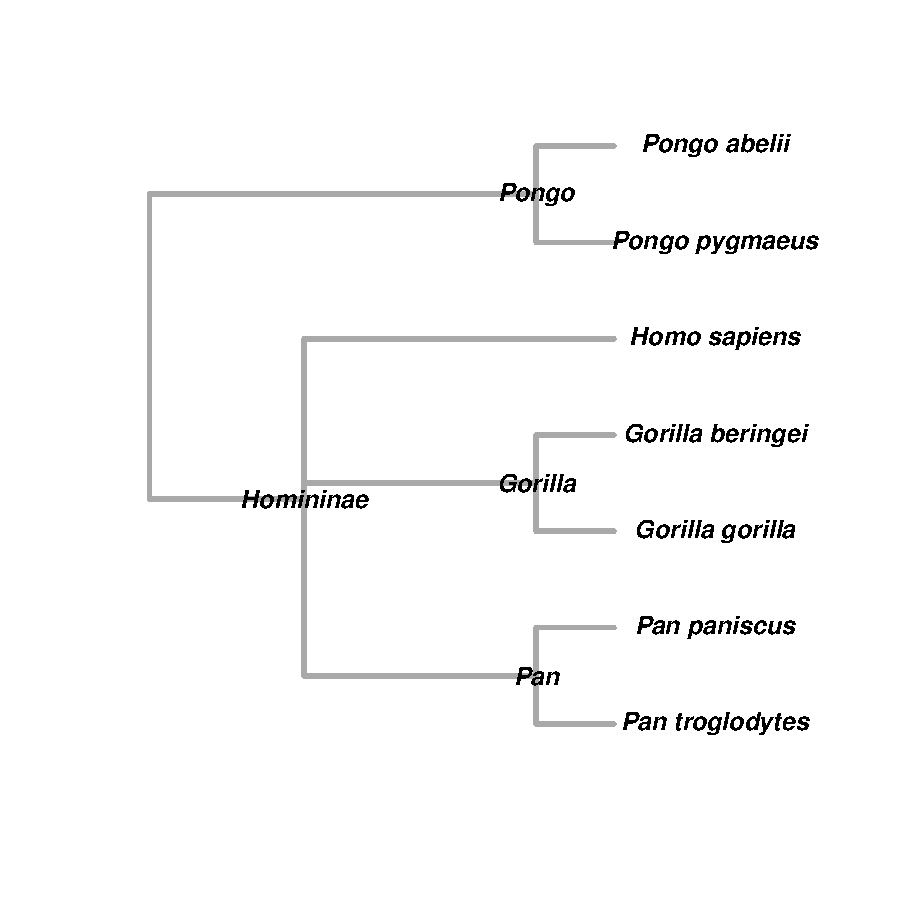
\includegraphics{ReolUserManual-014}
\end{center}

There are a few options available for creating the tree.  First, the argument includeNodeLabels will write node labels to the tree file a component of the class phylo.  You can see these in the same way as viewing other pieces of the tree object.  You can choose to turn this off if you will be creating edge labels for the tree anyway or just don't care to label anything.  It will take up some computational time depending on how big the tree is, so if you don't plan to label, then it is best to turn them off.  Second, because EOL data can be so easily downloaded and these downloaded files can be of any hierarchical rank, we needed a way to build a tree with missing data.  For example, if several taxa are genera and the rest are species, how will the tips align in the tree?  In this case, you can set the missingData argument to either prune the taxa with the missing information or you can prune the ranks without the information.  In either case, this will not be necessary if all the taxa are of the same rank.  Third, a user can predefine the rankings to use when building the tree, for example if you would like the tree to be build using only the taxon phylum, class, and species you can set userRanks = c("Phylum", "Class", "Species") and it will only take these rankings into account.  Note that this option can change the tree topology!  

\textit{Reol} also has a function to create edge labels with the taxonomic group names automatically. In some cases there are multiple taxonomic names for one edge, and the user can choose whether to print the most recent divergence name, the oldest divergence name, or do a combined name that will display all the names.  In the same way as when making the tree, any missing tip taxon information will have to be dealt with using the argument missingData.  

There is a bit more flexibility with visualization using the edge label functions rather than the node label functions. 

\begin {center}
\begin{Schunk}
\begin{Sinput}
> MakeEdgeLabels(NCBIfiles, duplicateEdgeLabels="oldest")
\end{Sinput}
\begin{Soutput}
Homininae       Pan   Gorilla  Ponginae 
        1         2         5         9 
\end{Soutput}
\begin{Sinput}
> MakeEdgeLabels(NCBIfiles, duplicateEdgeLabels="recent")
\end{Sinput}
\begin{Soutput}
Homininae       Pan   Gorilla     Pongo 
        1         2         5         9 
\end{Soutput}
\begin{Sinput}
> MakeEdgeLabels(NCBIfiles, duplicateEdgeLabels="combined")
\end{Sinput}
\begin{Soutput}
     Homininae            Pan        Gorilla Ponginae.Pongo 
             1              2              5              9 
\end{Soutput}
\begin{Sinput}
> edges <- MakeEdgeLabels(NCBIfiles)
> plot(ApeTree, "c", show.node.label=FALSE)
> edgelabels(text=names(edges), edge=edges, bg="light gray")
\end{Sinput}
\end{Schunk}
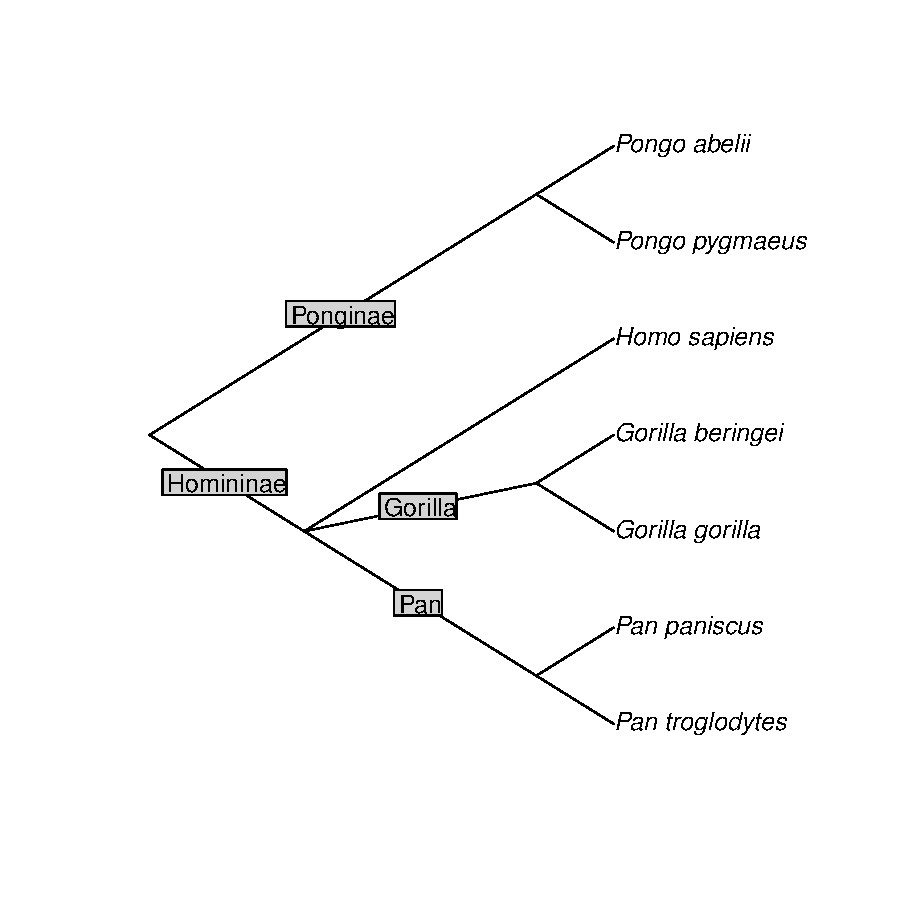
\includegraphics{ReolUserManual-015}
\end{center}

These trees can be used to plot information about EOL data. For example, if we want to know patterns of the number of common names across our taxa, we can plot that information as a continuous trait along our new taxonomy tree. One word of caution is to use \textit{Reol's} matching functions when plotting text on a tree.  This is especially true when plotting EOL data on a provider hierarchy tree, since the two may not overlap in taxon names or even number of files.  The first matching function is \code{MatchHierPageToEOLdata}, which will create a table of data with hierarchy/provider IDs and their associated EOL data.  We recommend that if you are going to be traversing EOL and Hier pages that you go through this function, since it will match up unique IDs rather than taxon names.  

The second matching function is to aid in plotting data on the taxonomic tree.  Tips in the tree are labeled according to their order in tip.labels, which likely will not match up with the order of your EOL input files.  There are different ways that you can ensure plotting the correct data with its matching tip (for example plotting each tip at a time), however the function \code{MatchDataToTreeTips} will do it automatically.  This function creates a new table, where each row is a tip taxon and data gets populated to that row in the correct order (if no data exists for that tip, then it is left as NA as a place holder).  For this function, you will need a tree and data that contains hierIDs, either data scraped from the hierarchy pages OR EOL data that has been matched using the function \code{MatchHierPageToEOLdata}.  

\begin{Schunk}
\begin{Sinput}
> MatchHierPageToEOLdata(MyHiers, GetRichnessScores(DownloadedApes))
\end{Sinput}
\begin{Soutput}
                         HierID  eolID Richness_Score
Camelus bactrianus     51377077 344581           <NA>
Camelus dromedarius    51377078 309019           <NA>
Hippopotamus amphibius 51377070 311532           <NA>
Rattus rattus          51380078 328447           <NA>
Rana cascadae          51349060 330264           <NA>
Bufo bufo              51345859 333310           <NA>
\end{Soutput}
\begin{Sinput}
> MatchDataToTreeTips(ApeTree, MatchHierPageToEOLdata(MyHiers, 
+      GetRichnessScores(DownloadedApes)))
\end{Sinput}
\begin{Soutput}
                 HierID eolID Richness_Score
Pan troglodytes      NA    NA             NA
Pan paniscus         NA    NA             NA
Gorilla gorilla      NA    NA             NA
Gorilla beringei     NA    NA             NA
Homo sapiens         NA    NA             NA
Pongo pygmaeus       NA    NA             NA
Pongo abelii         NA    NA             NA
\end{Soutput}
\begin{Sinput}
> MatchDataToTreeTips(ApeTree, GatherSynonyms(NCBIfiles, "c"))
\end{Sinput}
\begin{Soutput}
                            Taxon   hierID NumberOfSynonyms
Pan troglodytes   Pan troglodytes 51378532                0
Pan paniscus         Pan paniscus 51378531                0
Gorilla gorilla   Gorilla gorilla 51378523                0
Gorilla beringei Gorilla beringei 51378527                0
Homo sapiens         Homo sapiens 51378539                0
Pongo pygmaeus     Pongo pygmaeus 51378544                0
Pongo abelii         Pongo abelii 51378546                2
\end{Soutput}
\end{Schunk}

A simple example of plotting data.  In this example, we are plotting the number of English common names for each Great Ape species.  
\begin {center}
\begin{Schunk}
\begin{Sinput}
> CNs <- GetCommonNames(DownloadedApes, output="c")
> plot(ApeTree, label.offset=0.5, x.lim=10, no.margin=TRUE)
> edgelabels(text=names(edges), edge=edges, bg="light blue")
> trans <- CNs[,3]/10
> matched <- MatchDataToTreeTips(ApeTree, MatchHierPageToEOLdata(MyHiers, CNs))
> tiplabels(pch=22, bg=rgb(0,0.5,0.5,trans), cex=2.8, adj=0.7)
> tiplabels(matched[,3], frame="none", bg="clear",adj=-1)
\end{Sinput}
\end{Schunk}
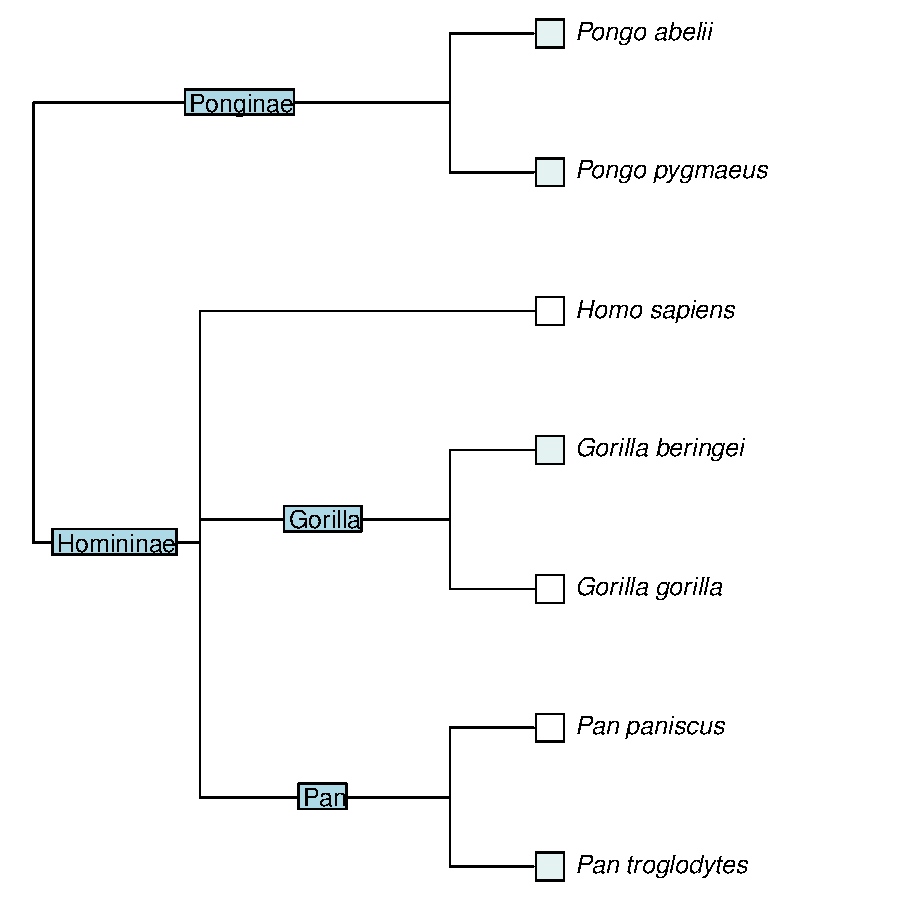
\includegraphics{ReolUserManual-017}
\end{center}

 
Another simple example of plotting data.  In this example, we are plotting the IUCN status for each Great Ape species.  
 \begin {center}
\begin{Schunk}
\begin{Sinput}
> ApeData <- MatchDataToTreeTips(ApeTree, 
+      MatchHierPageToEOLdata(NCBIfiles, GetIUCNStat(DownloadedApes)))
>   for(i in sequence(dim(ApeData)[1])) {
+     if(ApeData[i,3] == "Least Concern (LC)") {
+       ApeData[i,4] <- "Khaki"
+       ApeData[i,5] <- "LC"
+     }  
+     else if(ApeData[i,3] == "Endangered (EN)") {
+       ApeData[i,4] <- "Goldenrod"
+       ApeData[i,5] <- "EN"
+     }
+     else if(ApeData[i,3] == "Critically Endangered (CR)") {
+       ApeData[i,4] <- "coral4"
+       ApeData[i,5] <- "CR"
+     }
+   }
> plot(ApeTree, label.offset=0.8, x.lim=11)
> edgelabels(text=names(edges), edge=edges, bg="DarkGray")
> tiplabels(pch=21, bg=ApeData[,4], cex=4, adj = 0.85)
> tiplabels(ApeData[,5], frame="none", bg="clear",adj = -0.3)
> title(main="IUCN Status")
\end{Sinput}
\end{Schunk}
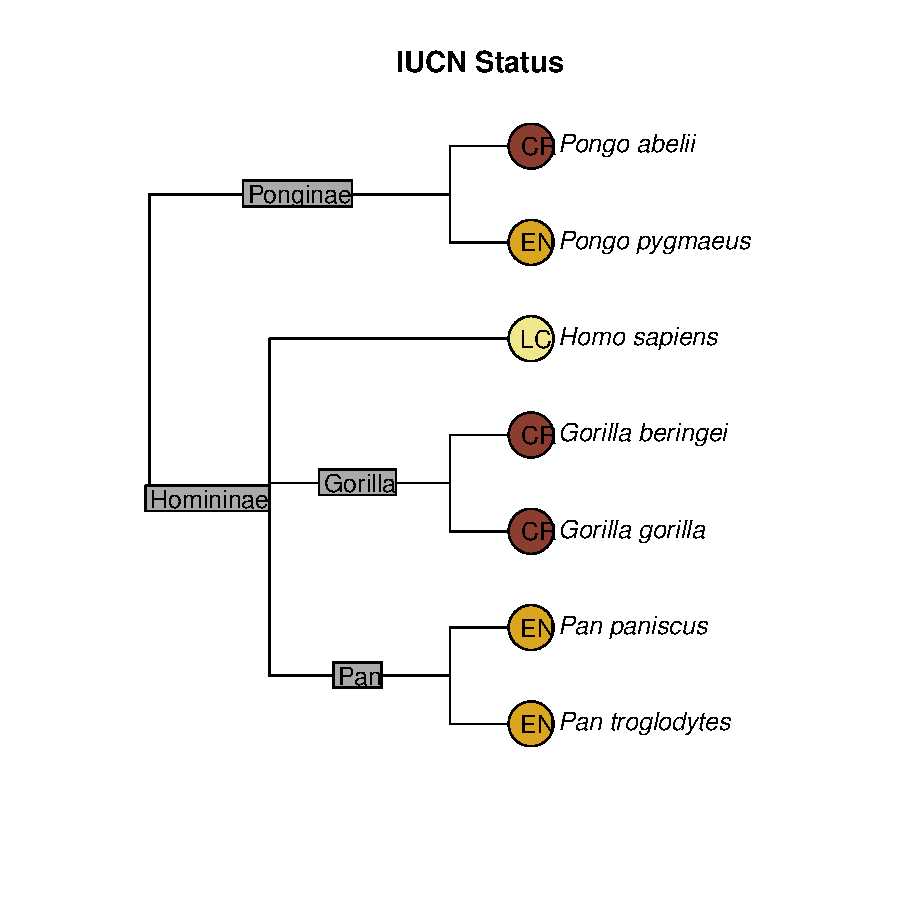
\includegraphics{ReolUserManual-018}
\end{center}

 
 
\end{document}




































